\documentclass[../../dissertation.tex]{subfiles}
\begin{document}

\subsection{Grover}
As was seen in section \ref{sec:chapGrover}, Grover's algorithm is a quantum alternative to unstructured search problems. Consider the case of finding element $x_0$ out of an unordered list of size $N$. Worst case scenario, a classical algorithm would need to check every element of the list, requiring $N$ steps.\par
The first stage of Grover's algorithm is to create an uniform superposition of all states in the system
\begin{equation}
	\ket{\Psi_0}  = \frac{1}{\sqrt{N}}\sum_{x=0}^{N-1} \ket{x}.
\end{equation}
Next is the application of the Grover iteration process, which starts with an oracle that adds a negative phase to the solution states
\begin{equation}
        \mathcal{O}\ket{x} = (-1)^{f(x)}\ket{x}.
\end{equation}
This operator can be seen as an identity matrix with negative entries corresponding to the solution states, and the operator can be rewritten as 
%TODO: Reescrever com o somatorio dos estados marcados?
\begin{equation}
	\mathcal{O} = I - 2\sum_{m\in M} \ket{m}\bra{m}.
	\label{eq:groverQiskitOracle}
\end{equation}
where $I$ is the identity matrix and $M$ is a set of solutions where $f(m) = 1$, otherwise it's $0$. The matrix associated with this operator will be
\begin{equation}
	\mathcal{O} = 
	\begin{pmatrix}
		(-1)^{f(0)} & 0 & \cdots & 0\\
	        0 & (-1)^{f(1)} & \cdots & 0\\ 
	        \vdots & 0 &  \ddots & \vdots\\ 
		0 & 0 & \cdots &  (-1)^{f(N-1)}
	\end{pmatrix}.
	\label{eq:oracleMatrixQiskit}
\end{equation}
%TODO: Mencionar que o grover se extende a toda a categoria de problemas que envolvam aquela matriz.
The second part of the iteration is an amplitude amplification process by means of the diffusion operator 
\begin{equation}
        %TODO: Decidir se mantenho os H's.
        \mathcal{D} = (2\ket{\Psi_0}\bra{\Psi_0} - I) = H^{\otimes n}(2\ket{0}\bra{0} - I)H^{\otimes n}.
	\label{eq:groverQiskitDiffusion}
\end{equation}
The unitary operator that describes the Grover iteration process will then be
\begin{equation}
        \mathcal{U} = \mathcal{D}\mathcal{O}.
\end{equation}\par
As was shown in section \ref{sec:chapGrover} this iteration process will be done several times, depending on the number of elements. Optimal probability of success finding a single solution will be reached after $\floor{\frac{\pi}{4}\sqrt{N}}$ steps, and $\floor{\frac{\pi}{4}\sqrt{\frac{N}{K}}}$ for $K$ solutions, which is a quadratic gain when compared to the classical case. The circuit can then be constructed as is shown in figure \ref{}.
\begin{figure}[!h]
	\[ \Qcircuit @C=1.8em @R=1.5em {& & & && \mbox{ Repeat $O(\sqrt{N})$ times}  & & &\\
	& & {/^{\otimes n}} \qw &\gate{H}  & \gate{\mathcal{O}} &  \gate{D} & \qw &\qw \gategroup{2}{5}{2}{6}{.8em}{--}
		          } \]
	\centering
	\caption{Temp}
	\label{fig:groverSearchCircuit}
\end{figure}\par
Consider the $3$ qubit case, where $N=8$ and solution state $\ket{4}$. The optimal number of iterations is approximately $2$, and figure \ref{fig:groverCircuitQistkit} is the circuit for $3$ iterations implemented in Qiskit.
\begin{figure}[!h]
	\centering
	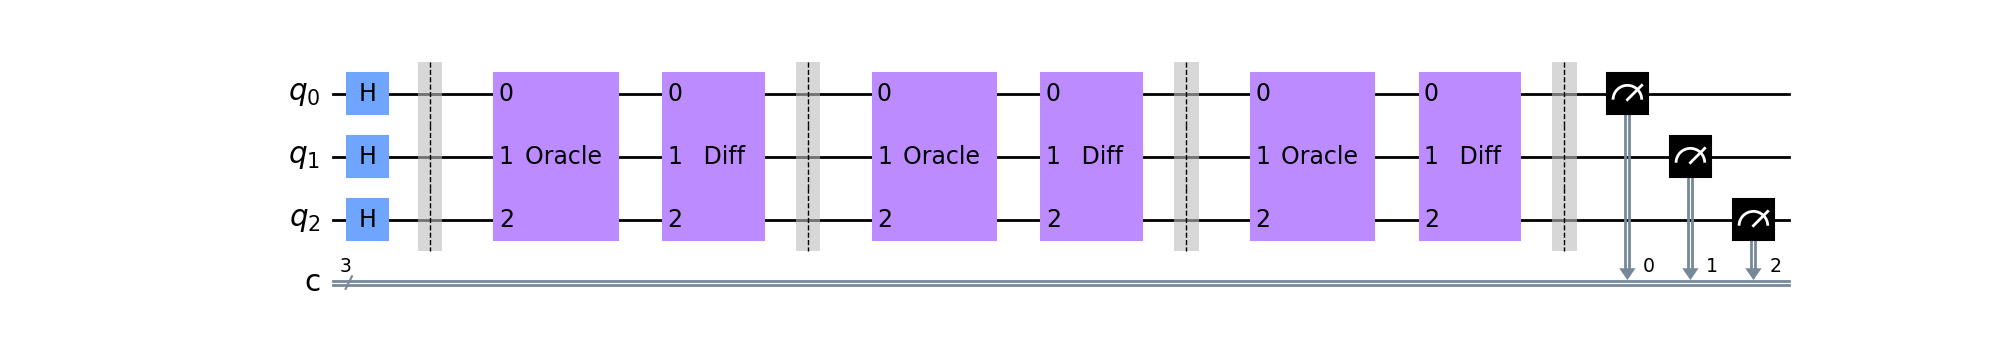
\includegraphics[scale=0.32]{img/Qiskit/GroverQiskit/Circuits/GroverQiskitCirc_N3_M4_S3.png}
	\caption{Temp}
	\label{fig:groverCircuitQistkit}
\end{figure}\par
%TODO:Melhorar 
The system starts with the creation of an uniform superposition state, which means applying Hadamard gates to each qubit. 
\begin{figure}[!h]
	\centering
	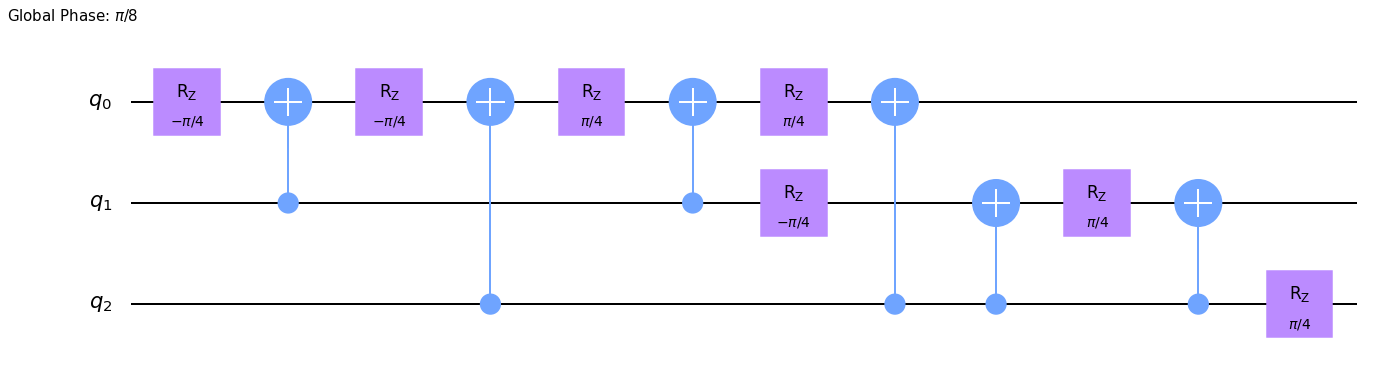
\includegraphics[scale=0.25]{img/Qiskit/GroverQiskit/Circuits/GroverQiskitCircOracle_N3_M4_S3.png}
	\caption{Temp}
	\label{fig:groverOracleCircuitQistkit}
\end{figure}
Immediately following the barrier, the first operator of the iteration process is the oracle, which is shown in figure \ref{fig:groverOracleCircuitQistkit}. 
Because the oracle operator is simply the identity matrix with negative entries corresponding to the solution states, it can be simply translated into a circuit by means of the diagonal function in Qiskit. The last part of the iteration is the diffusion operator, whose circuit is shown in figure \ref{fig:groverDiffCircuitQistkit}.

\begin{figure}[!h]
	\centering
	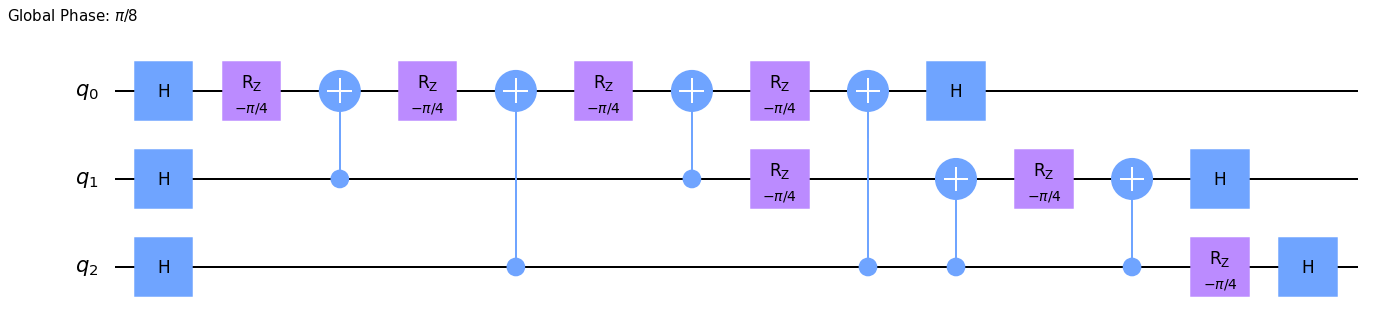
\includegraphics[scale=0.25]{img/Qiskit/GroverQiskit/Circuits/GroverQiskitCircDiff_N3_M4_S3.png}
	\caption{Temp}
	\label{fig:groverDiffCircuitQistkit}
\end{figure}
%TODO Isto esta muito fraco. 
Comparing equations \ref{eq:groverQiskitOracle} and \ref{eq:groverQiskitDiffusion}, it is easy to see why figures \ref{fig:groverOracleCircuitQistkit} and \ref{fig:groverDiffCircuitQistkit} are very similar. The diffusion circuit will simply be the oracle circuit for state $\ket{0}$ in between Hadamard operations.

\begin{figure}[!h]
	\centering
	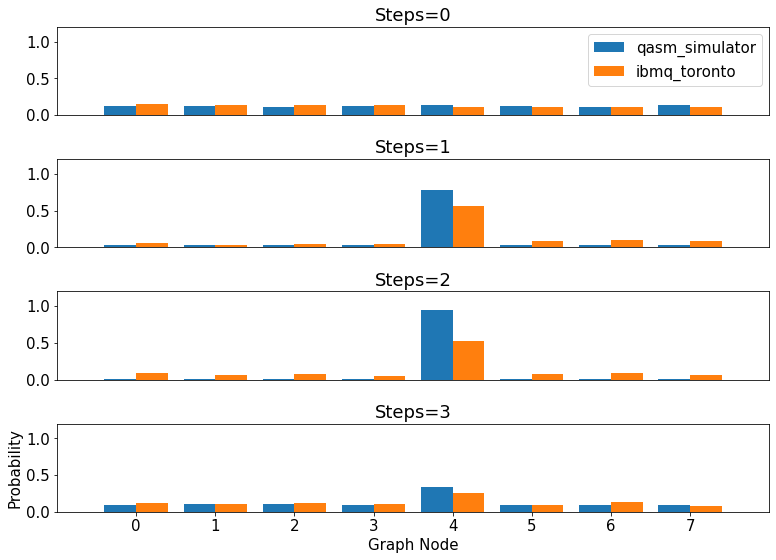
\includegraphics[scale=0.40]{img/Qiskit/GroverQiskit/GroverQiskitSearch_N3_M4_S0123}
	\caption{Temp}
	\label{fig:groverQiskitDist}
\end{figure}
%TODO: Escrever mais
The results of measurement are shown in figure \ref{fig:groverQiskitDist}. As was expected, maximum probability for the marked element was reached after $2$ iterations, on the simulator, and it decreases in subsequent steps. However, the experimental result from the Toronto backend present maximum probability for the marked element for $1$ step, with a fidelity of $0.96$, and a fidelity of $0.89$ for the optimal number of steps steps. This is because as the number of steps increases, so does circuit depth, meaning that the circuit does not achieve the maximum probability after $2$ steps due to the effects introduced by noise.\par
The results, however, are satisfactory when considering the properties of NISQ computers. The next sections will present the search problem when considering several quantum walk models, sorted by their feasibility on noisy quantum hardware. 

\subsection{Coined}
As previously done in section \ref{sec:chap3CoinedSearch}, this chapter aims to expand the coined quantum walk model incorporating concepts like the oracle and diffusion operator of the Grover algorithm. In fact, for the complete graph case, the coined quantum walk and Grover's algorithm are equivalent.\par
The modified unitary evolution operator is
\begin{equation}
        U' = S (\mathcal{O} \otimes G),\label{eq:modifiedEvoCoinedQiskit}
\end{equation}
%TODO: Relembrar equacoes para cada um dos operadores? Parece me desnecessario.
as was defined in equation \ref{eq:modifiedEvoCoined}, where $S$ is the flip-flop shift operator, $\mathcal{O}$ is the oracle operator and $G$ is the Grover diffusion as a coin operator.\par
Consider the case of a complete graph, where every vertex is adjacent to one another. The quantum circuit to implement this, as shown in figure \ref{fig:coinedSearchCircuit}, will require $N$ qubits to represent the state of the walker and $N$ qubits for the state of the coin.  The shift operator was constructed based on the work of \cite{douglaswang07}, where the state of the walker is flip-flopped with the state of the coin, which can be done through swap gates.

\begin{figure}[!h]
	\[ \Qcircuit @C=1.8em @R=1.5em { & & & & \mbox{ Repeat $O(\sqrt{N})$ times}  &\\
	                                & {/^{\otimes n}} \qw  &\gate{H}  & \gate{\mathcal{O}} & \multigate{1}{SHIFT} & \qw &  \\
				                    & {/^{\otimes n}} \qw  & \qw & \gate{G}&   \ghost{SHIFT} & \qw \gategroup{2}{4}{3}{5}{.8em}{--}
		          } \]
	\centering
	\caption{Douglas wang coined quantum walk circuit}
	\label{fig:coinedSearchCircuit}
\end{figure}

\par
This was implemented in Qiskit, for a graph of size $N=2^3=8$, which means $6$ qubits will be required. For the case of one marked element, the number of iterations that maximizes the amplitude of the solution state is $\floor{\frac{\pi}{2} \sqrt{N}}$, and figure \ref{fig:coinedQWSearchCircuitQistkit}
shows the circuit for 5 iterations of the walk.
\begin{figure}[!h]
	\centering
	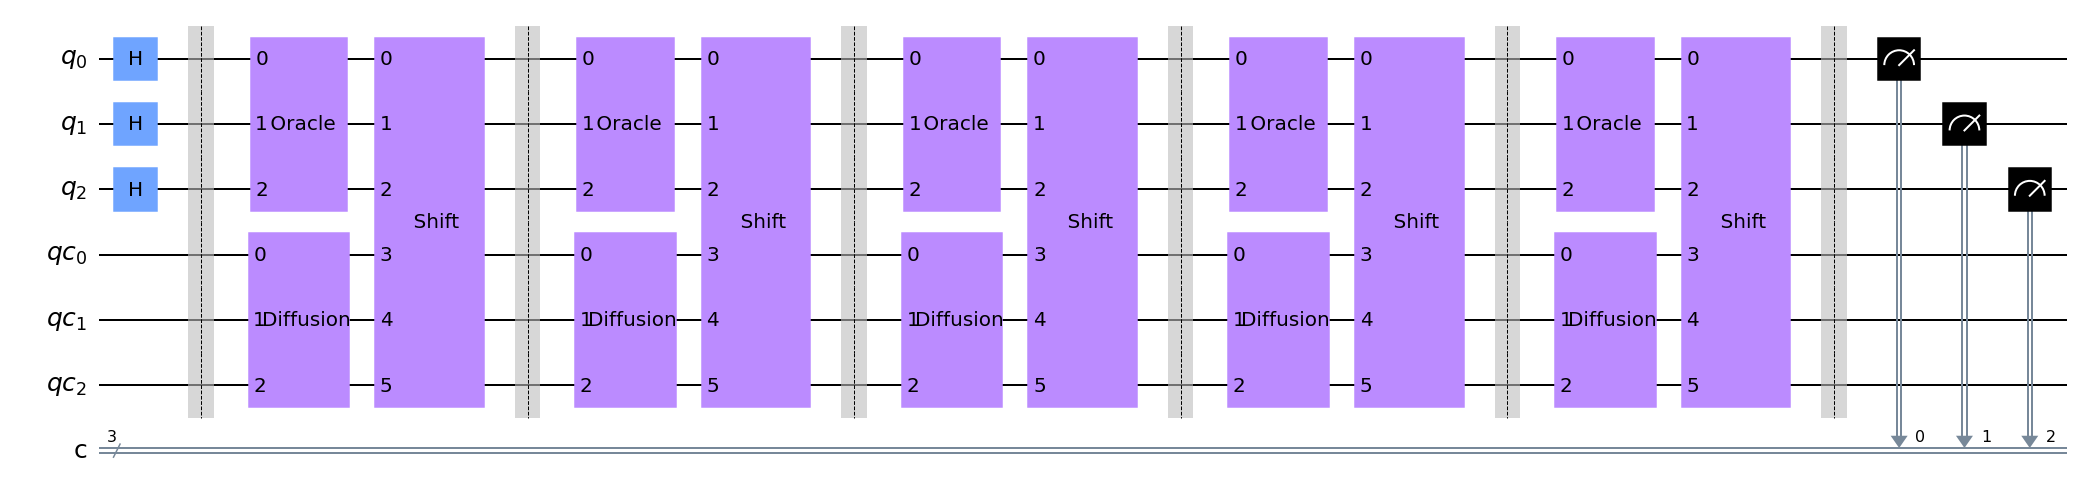
\includegraphics[scale=0.21]{img/Qiskit/CoinedQuantumWalk/Search/Circuits/CoinedSearchQiskitCirc_N3_M0_S5.png}
	\caption{Temp} 
	\label{fig:coinedQWSearchCircuitQistkit}
\end{figure}\par
The circuit starts in a uniform superposition of the states corresponding to the vertices of the graph, and the first step of the iteration is the oracle. This operator will flip the amplitude of the vertex state $\ket{4}$, and can be translated to a circuit making use of Qiskit's \textit{diagonal}, as is shown in figure \ref{fig:coinedQWSearchOracleCircuitQistkit}. It is the same operator as in figure \ref{fig:groverOracleCircuitQistkit}, and in the coined quantum walk model it is only applied to the states associated with the position of the walker.
\begin{figure}[!h]
	\centering
	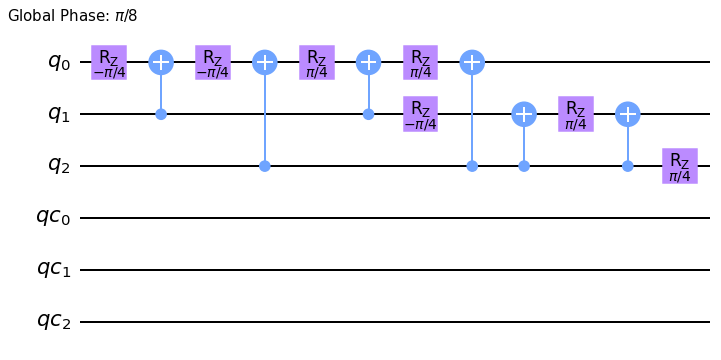
\includegraphics[scale=0.30]{img/Qiskit/CoinedQuantumWalk/Search/Circuits/CoinedSearchQiskitCircOracle_N3_M4_S5.png}
	\caption{Temp} 
	\label{fig:coinedQWSearchOracleCircuitQistkit}
\end{figure}
%TODO: Reescrever
The states associated with the coin space of the walk will be transformed according to Grover's diffusion, as is seen in figure \ref{fig:coinedQWSearchDiffCircuitQistkit}.
\begin{figure}[!h]
	\centering
	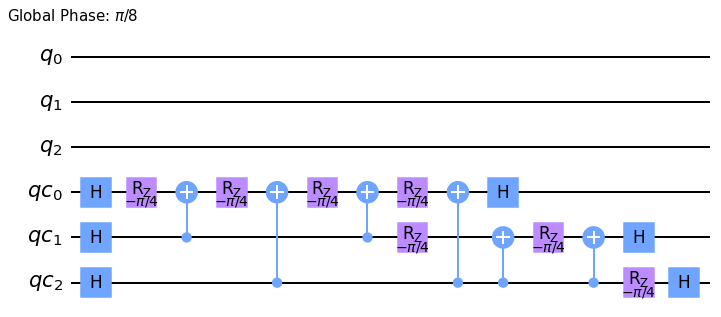
\includegraphics[scale=0.30]{img/Qiskit/CoinedQuantumWalk/Search/Circuits/CoinedSearchQiskitCircDiff_N3_M4_S5.png}
	\caption{Temp} 
	\label{fig:coinedQWSearchDiffCircuitQistkit}
\end{figure}
The final part of the iteration is the shift operator, as can be seen in figure \ref{fig:coinedQWSearchShiftCircuitQistkit}. The flip-flop shift operator was defined in equation \ref{eq:chap3FlipFlop} as 
\begin{equation}
        S\ket{v1}\ket{v2} = \ket{v2}\ket{v1},
        \label{eq:chap4FlipFlop}
\end{equation}
where $\ket{v1}$ represents the position of the walker and $\ket{v2}$ is the state of the coin. Making use of the swap gate, this operator can be implemented as in figure \ref{fig:coinedQWSearchShiftCircuitQistkit}.
\begin{figure}[!h]
	\centering
	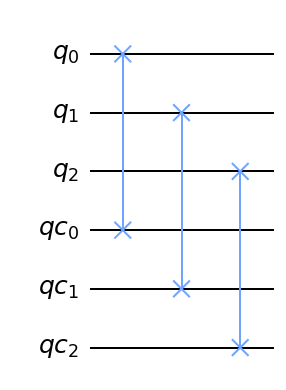
\includegraphics[scale=0.27]{img/Qiskit/CoinedQuantumWalk/Search/Circuits/CoinedSearchQiskitCircShift_N3_M4_S5.png}
	\caption{Temp} 
	\label{fig:coinedQWSearchShiftCircuitQistkit}
\end{figure}\par
%TODO: Estudar porque e que a dist muda logo para 0 (diffusion) em steps = 5
%TODO: Melhorar texto.
Lastly, measurements were performed, and the results plotted in figure \ref{fig:coinedSearchQiskitDist}. Maximum probability of the marked element was reached after $4$ steps in the simulator, and extra steps reduce said probability. 
\begin{figure}[!h]
	\centering
	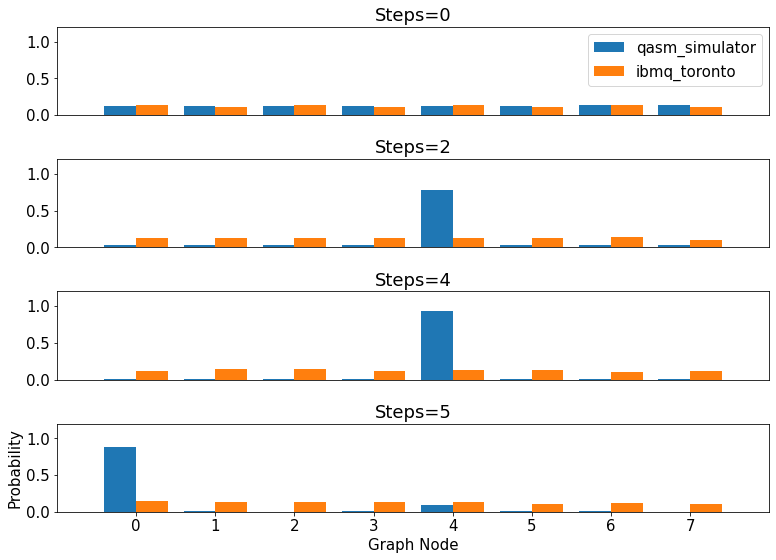
\includegraphics[scale=0.40]{img/Qiskit/CoinedQuantumWalk/Search/CoinedQiskitSearch_N3_M4_S0245}
	\caption{Temp } 
	\label{fig:coinedSearchQiskitDist}
\end{figure}
The resulting probability distribution from the Toronto backend is again unsatisfactory for the coined quantum walk model, with fidelities ranging from $0.58$ for $4$ steps, to $0.75$ for $2$ steps. This is expected, since the complete graph representation requires $N$ extra qubits for the coin, and swap operations which are decomposed into $3$ CNOTs each. The optimal number of steps that maximizes the probability of the marked element is also a contributing factor to the size of the circuit, requiring more iterations to achieve the same probability when compared to Grover's search in the previous chapter.\par
As was done previously, other models of the quantum walks that do not require coins or iterations will be studied in the following sections, in the context of the searching problem. The staggered quantum walk, for example, should be able to present better results when ran in a NISQ computer since it is a coinless model.

\subsection{Staggered}
Recalling from section \ref{sec:StagSearchSimul}, the staggered quantum walk on
a complete graph requires a single tessellation with associated polygon
\begin{equation}
	\ket{\alpha} = \frac{1}{\sqrt{N}} \sum_{x=0}^{N-1} \ket{x}.
\end{equation}
The Hamiltonian will then be 
\begin{equation}
	H_\alpha = 2\sum_0^1\ket{\alpha}\bra{\alpha} - I = H^{\otimes n} (2\ket{0}\bra{0} - I) H^{\otimes n} = H^{\otimes n} \mathcal{O}_0 H^{\otimes n},
\end{equation}
which is equivalent to the Grover diffusion operator, meaning it can be
implemented in a similar fashion. The evolution operator for the staggered
quantum walk on the complete graph will then be 
\begin{equation}
	U = e^{i\theta H_\alpha} = e^{i\theta(H^{\otimes n} \mathcal{O}_0 H^{\otimes n})} = H^{\otimes n} e^{i\theta\mathcal{O}_0} H^{\otimes n}.
	\label{eq:unmodEvolOperatorStagSearch}
\end{equation}
This is a very useful representation since the exponent part of the operator is
a diagonal matrix, which means implementing the circuit in Qiskit is a
straightforward task.\par 

Now that the staggered quantum walk associated with the
complete graph is defined, what remains is to add an oracle to the evolution
operator as was done in equation \ref{eq:stagSearchSimulModEvoOp},
\begin{equation}
        U' = U\mathcal{O},
        \label{eq:stagSearchQiskitModEvoOp}
\end{equation}
where
\begin{equation}
	\mathcal{O} = I_N - 2\sum_{m \in M}\ket{m}\bra{m},
\end{equation}
and $M$ is the set of marked elements.\par
The general circuit for implementing the staggered quantum walk search problem
in a complete graph will then be as shown in figure
\ref{fig:stagSearchCircuit}. 
\begin{figure}[!h]
	\[ \Qcircuit @C=1.8em @R=1.5em { &&&&& \mbox{Repeat $O(\sqrt{N})$ times.} & &\\
	& & {/^{\otimes n}} \qw& \gate{H} &\gate{\mathcal{O}} &\gate{H}  & \gate{e^{i\theta\mathcal{O}_0}} &  \gate{H} &\qw \gategroup{2}{5}{2}{8}{.8em}{--} \\
		          } \]
	\centering
	\caption{Temp}
	\label{fig:stagSearchCircuit}
\end{figure}
Since only one tesselation is required, there is no need for the Suzuki-Trotter
aproximation. However, several iterations will be needed in order to achieve
maximum probability for the marked vertex. Because the staggered quantum walk
search on a complete graph is equivalent to Grover's algorithm, the optimum
number of steps will also be $\frac{\pi}{4}\sqrt{\frac{N}{K}}$, where K is the
number of solutions.\par
%TODO: Definir para todas as walks N grande = numero total de elementos e n pequeno = numero de qubits.
Consider the case of $N=8$ and one marked vertex, $\ket{m}=\ket{4}$. The number of steps
that maximizes the probability of the marked element is
$\frac{\pi}{4}\sqrt{\frac{8}{1}} \approx 2$. Translating to Qiskit, $n=3$
qubits will be needed and the circuit will be as in figure \ref{fig:stagSearchCircQistkit}. 

\begin{figure}[!h]
	\centering
	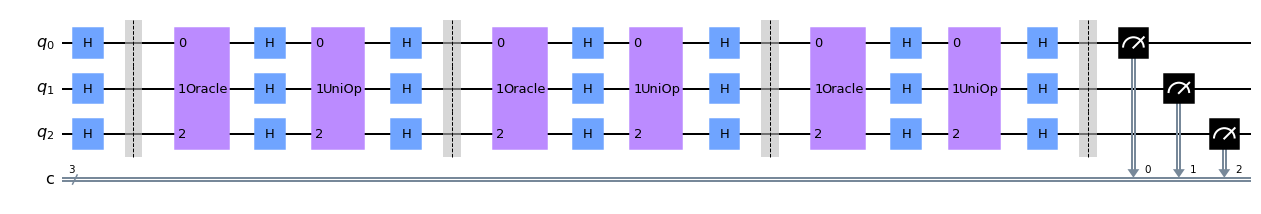
\includegraphics[scale=0.35]{img/Qiskit/StaggeredQW/Search/Circuits/StagSearchCircuit_N3_M0_S3.png}
	\caption{Temp}
	\label{fig:stagSearchCircQistkit}
\end{figure}
Similar to previous examples, the circuit begins with the uniform superposition
achieved through Hadamard gates. The next operation of the search problem is
the oracle, which was implemented through the use of Qiskit's \textit{diagonal}
function that produces a circuit similar to the one in figure
\ref{fig:groverOracleCircuitQistkit}. Next, an analogue of Grover's diffusion
operator is applied, where the operation named \textit{UniOp} is a diagonal
matrix, easily translated to Qiskit as is shown in figure
\ref{fig:stagSearchUniOpCircQistkit}.  
\begin{figure}[!h]
	\centering
	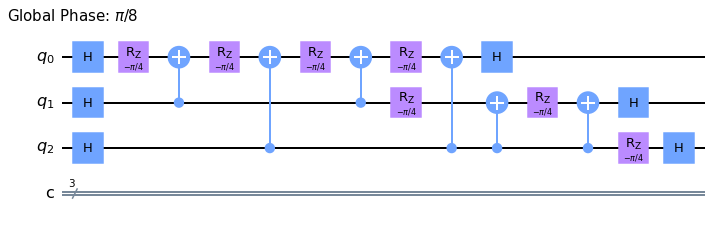
\includegraphics[scale=0.40]{img/Qiskit/StaggeredQW/Search/Circuits/StagUniOpCircuit_N3_M0_S3.png}
	\caption{Temp}
	\label{fig:stagSearchUniOpCircQistkit}
\end{figure}
This circuit is very similar to the one in figure
\ref{fig:groverDiffCircuitQistkit}, the difference being that in the staggered
quantum walk search model one can control the value of $\theta$, as can be seen
in equation \ref{eq:unmodEvolOperatorStagSearch}, which influences how fast
maxmimum probability of the marked element is achieved. Since Grover's
algorithm is optimal, a value of $\theta=\frac{\pi}{2}$ yields a diffusion
circuit equal to the one in figure \ref{fig:groverDiffCircuitQistkit}, implying
that the staggered quantum walk is a more general model of quantum searching.
Finally, measurement is performed and the resuls for several steps of the walk
are shown in figure \ref{fig:stagSearchResultsToronto}.  
\begin{figure}[!h]
	\centering
	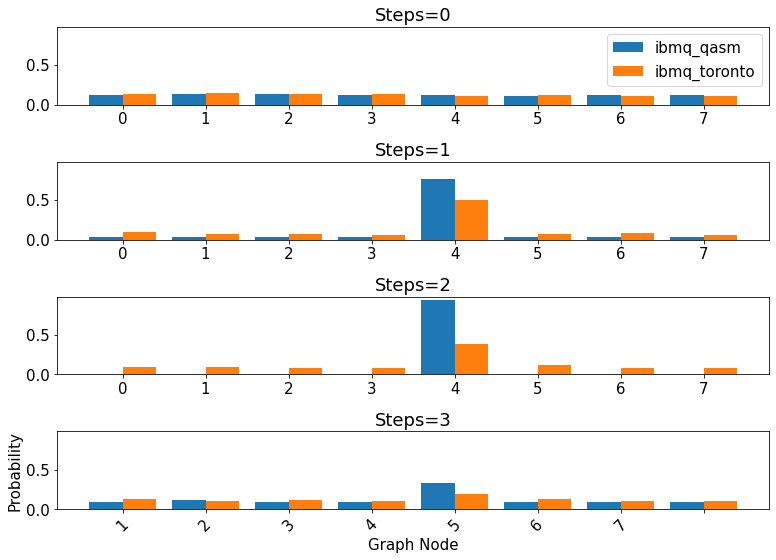
\includegraphics[scale=0.40]{img/Qiskit/StaggeredQW/Search/stagSearchToronto_N3_S0123.png}
	\caption{Temp}
	\label{fig:stagSearchResultsToronto}
\end{figure}
The circuit for each step of the walk was run both in the \textit{Qasm}
simulator and IBM's backend named Toronto. The experiment was performed with
$3000$ shots in both cases, and the probability distributions show that this model is indeed more suited for a NISQ computer than the previous case. However, unlike the simulator, maximum probability of the marked vertex was achieved
withing $1$ step of the walk instead of the predicted $2$ steps, as was the case of the Grover algorithm. Looking at the $1$ step case in the simulator, one can see that the probability of vertex $\ket{4}$ is very close to the maximum, while the circuit has about half of the operations of the $2$ step case. This means it is not surprising that the smaller circuit produces higher results for the probability of the marked vertex. 
%TODO: Talvez melhorar as fidelidades com o intervalo de confianca.
%TODO: Definir a metrica para fidelidade.
This can be further confirmed by the fidelities of each of the states,
which are aproximately $0.954$ and $0.780$ for $1$ step and $2$ steps,
respectively, implying that the former circuit produces better results because
of the number of operations, even though that the latter should theoretically
yield the highest probability.\par
Even though these results are a great improvement to the search problem using the coined quantum walk, the staggered model is still discrete, meaning it's circuit will increase in size as the number of steps increases. This can be avoided by turning again to the continuous-time model, whose circuit will not increase as time increases, but will need iterations due to the Suzuki-Trotter approximation, which was not the case in section \ref{sec:ContQiskit} where the searching problem was not a factor.

%TODO: Fazer com outra moeda usando u3 com valores intermedios entre pi/2 ou pi/4
\subsection{Continuous}
As was seen in section \ref{sec:chap3ContSearch}, the unitary operator associated with the continuous time quantum walk model can be modified as to mark an element for amplitude amplification
\begin{equation}
	U'(t) = e^{iH't} = \phi(t)e^{-i\gamma(A+O)t},
	\label{eq:qiskitU'}
\end{equation}
where $\phi(t)$ is a global phase, $A$ is the adjacency matrix and the oracle is defined as 
\begin{equation}
	O = \sum_{m \in M} \ket{m}\bra{m},
\end{equation}
where $M$ is the set of marked elements.\par
%TODO: !!ESCREVER MATRIZ ADJACENCIA GRAFO COMPLETO !!
This section will focus on constructing and analyzing the circuit form of the continuous-time quantum walk search problem, and the first step is to borrow the diagonal definition of the adjacency matrix from equation \ref{eq:qiskitContQWAdj} 
\begin{equation}
    A = F^{\dagger} \Lambda F,
    \label{eq:qiskitContSearchAdj}
\end{equation}
and use the Suzuki-Trotter expansion
\begin{equation}
	e^{i(H_0+H_1)t}=\lim_{n \rightarrow \infty}(e^{i\frac{H_0t}{n}}e^{i\frac{H_1t}{n}})^n ,
\end{equation}
to decompose the operator in equation \ref{eq:qiskitU'}
\begin{equation}
	e^{i\gamma(A+O)t} =\lim_{n \rightarrow \infty}(F^{\dagger} e^{i\gamma\frac{\Lambda t}{n}} F e^{i\gamma\frac{Ot}{n}})^n, 
	\label{eq:suzTrotter}
\end{equation}
which can be easily translated into circuit form as in figure \ref{fig:contSearchCircuit}. 
\begin{figure}[!h]
	\[ \Qcircuit @C=1em @R=1.0em {& & & & & \mbox{Repeat n times} & &\\
	&\lstick{\ket{qv^{\otimes n}}} & {/} \qw &\gate{H^{\otimes n}}  & \gate{e^{i\gamma\frac{Ot}{2}^{\otimes n}}} & \gate{F^{\otimes n}} &\gate{e^{i\gamma\frac{\Lambda t}{2}^{\otimes n}}} & \gate{F^{\dagger}} &\qw \gategroup{2}{5}{2}{8}{.8em}{--}
		          } \]
	\centering
	\caption{Temp}
	\label{fig:contSearchCircuit}
\end{figure}\par
Consider the case of a graph of size $N=3$ and trotter number of $n=2$. The corresponding Qiskit circuit is as shown in figure \ref{fig:contSearchCircuit}. The system starts out in an uniform superposition followed by a state transformation according to the oracle operator that can be seen in figure \ref{fig:contSearchOracleCircQistkit}. Note that the circuit was obtained by using the Qiskit diagonal function that takes the diagonal entries of the operator corresponding to the oracle, as in equation \ref{eq:suzTrotter}. 
\begin{figure}[!h]
	\centering
	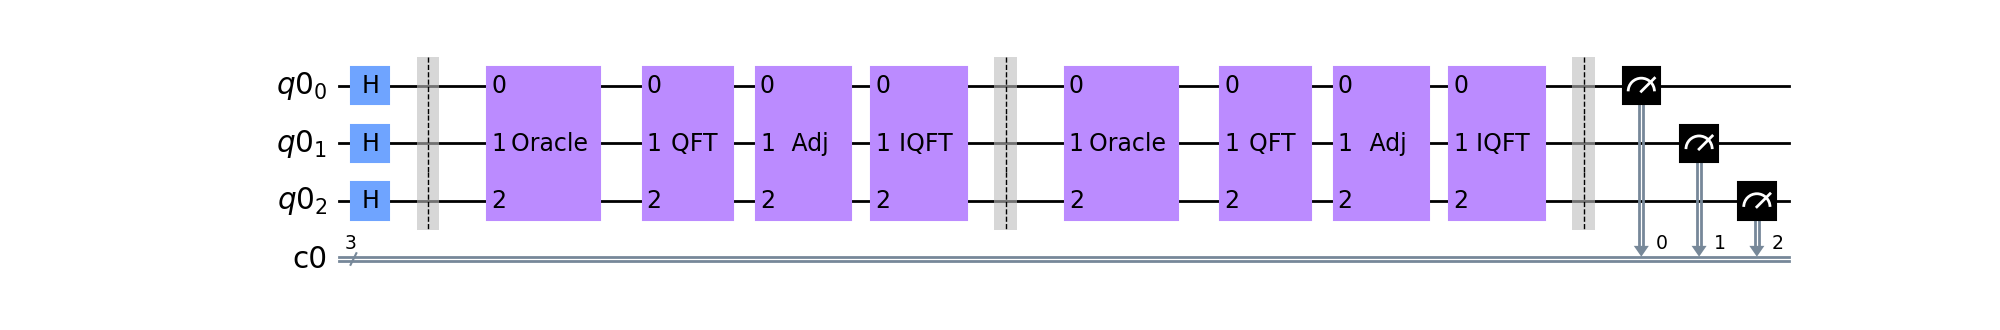
\includegraphics[scale=0.34]{img/Qiskit/ContQuantumWalk/Search/Circuits/circContSearch_N3_S2.png}
	\caption{Temp}
	\label{fig:contSearchCircQistkit}
\end{figure}
%TODO: Escrever mais sobre a adjacencia.
The following transformations will be the quantum Fourier transform, which is the same as in figure \ref{fig:qftCircuitQiskit}, and the operator associated with the adjacency matrix. Since $A$ is the diagonal adjacency matrix of a complete graph, it is easily implemented using Qiskit, as can be seen in figure \ref{fig:contSearchAdjCircQistkit}.
\begin{figure}[!h]
	\centering
	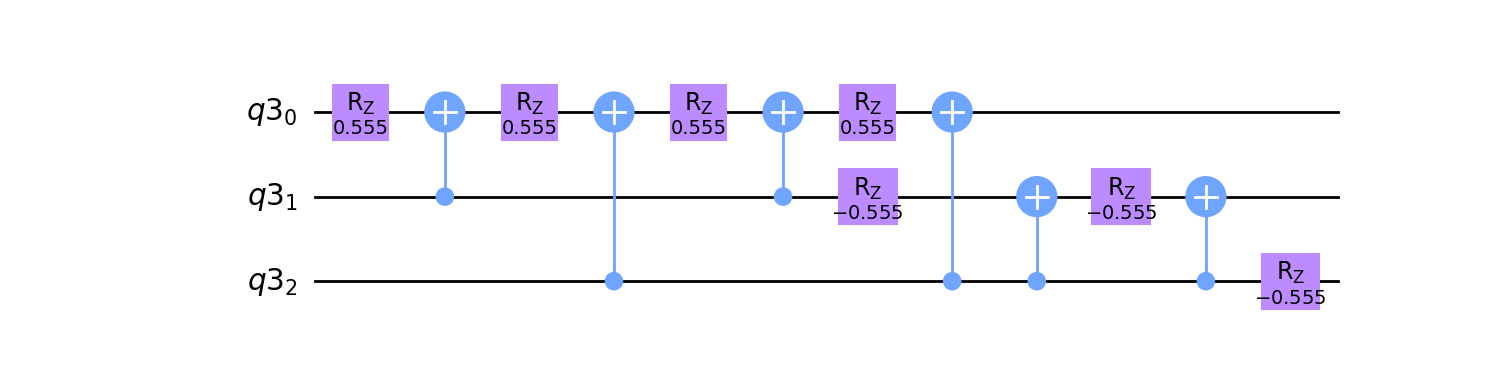
\includegraphics[scale=0.34]{img/Qiskit/ContQuantumWalk/Search/Circuits/circOracle_N3_S2.png}
	\caption{Temp}
	\label{fig:contSearchOracleCircQistkit}
\end{figure}
\par
%TODO: Escrever mais sobre resultados.
The results of measurement are shown in figure \ref{fig:contSearchResultCircQistkit}. 

\begin{figure}[!h]
	\centering
	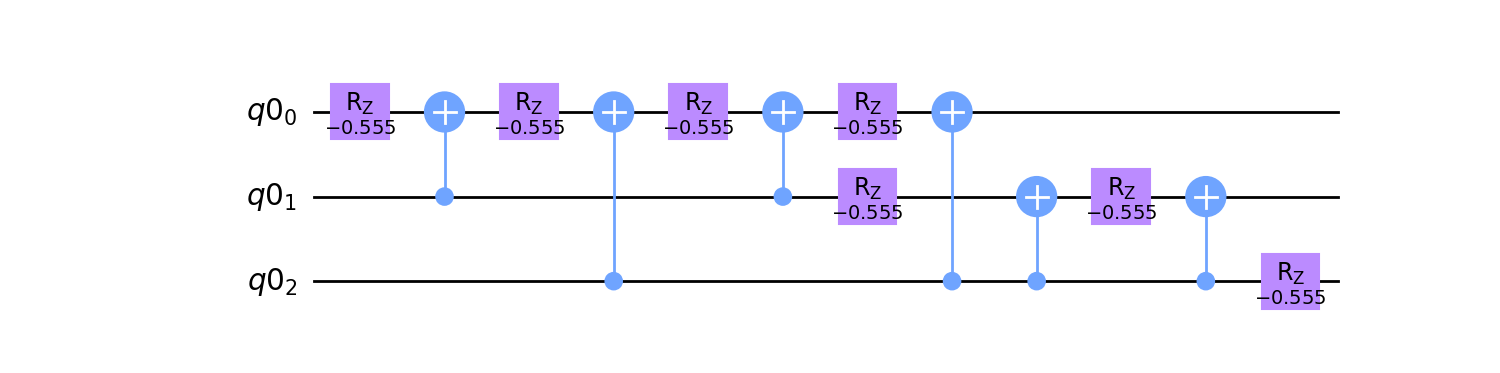
\includegraphics[scale=0.34]{img/Qiskit/ContQuantumWalk/Search/Circuits/circAjd_N3_S2.png}
	\caption{Temp}
	\label{fig:contSearchAdjCircQistkit}
\end{figure}

\begin{figure}[!h]
	\centering
	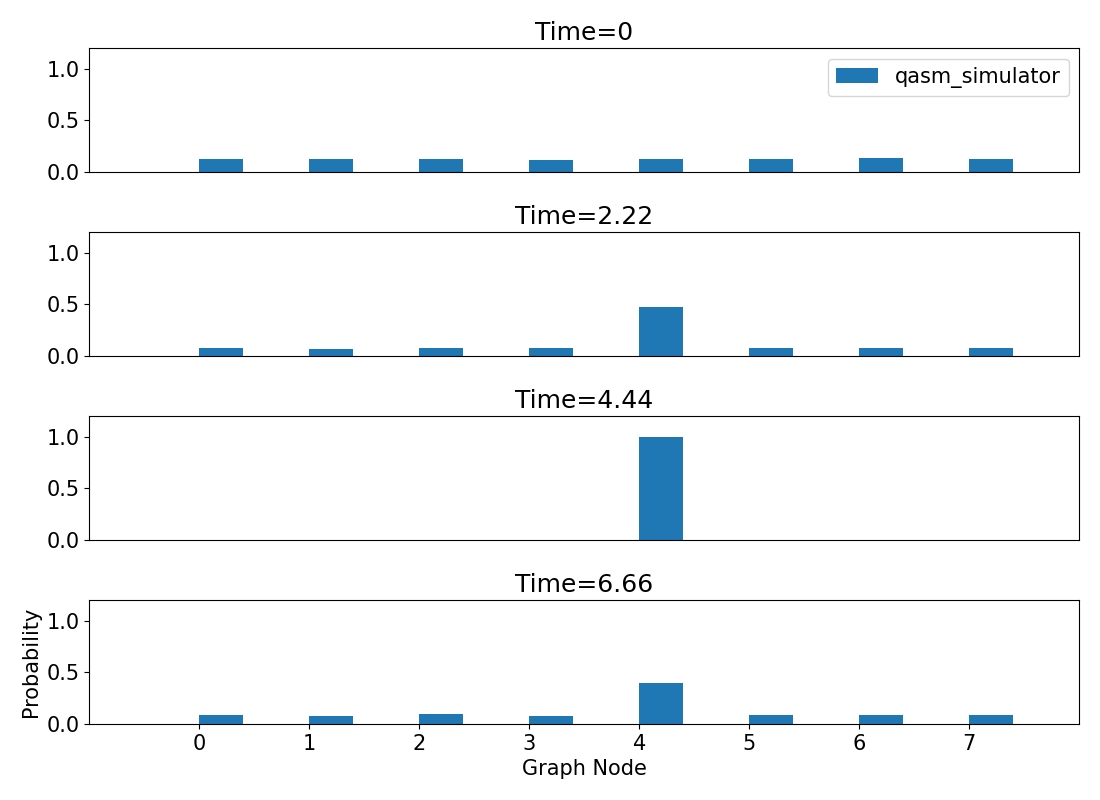
\includegraphics[scale=0.40]{img/Qiskit/ContQuantumWalk/Search/ContQW_N3_S2.png}
	\caption{Temp}
	\label{fig:contSearchResultCircQistkit}
\end{figure}

\end{document}
